\documentclass[xcolor=table]{beamer}
\usepackage[utf8]{inputenc}
\usepackage{default}
\usepackage{xspace,setspace}
\usepackage{amsmath,amsthm,amssymb}
\usepackage{ellipsis}
\usepackage[pdftex]{epsfig}
\usepackage{listliketab}
\usepackage[table]{xcolor}
\usepackage{booktabs}

\usepackage{pgf}
\usepackage{tikz}
\usetikzlibrary{arrows,automata}
\usetikzlibrary{graphs}
\tikzset{
     mainNode/.style =
        { circle
        , draw
        %, fill=blue!20,
        %, font=\sffamily\Large\bfseries
        }
}


%\usetheme{Berlin}
%\usetheme{Bergen}
%\usetheme{Antibes}
%\usetheme{Goettingen}
%\usetheme{Warsaw}
%\usetheme{Darmstadt}
%\usetheme{JuanLesPins}
%\setbeamertemplate{navigation symbols}{}

%\usecolortheme{beaver}
%\usecolortheme{rose}
%\usecolortheme{seagull}
%\usecolortheme{dove}
%\usecolortheme{seahorse}

%\usepackage{color,colortbl}
%\usepackage{texnansi}
%\usepackage{marvosym}
%\usepackage{comment}


\setbeamertemplate{frametitle}
{\begin{centering}\smallskip
   \insertframetitle\par
   \smallskip\end{centering}}
\setbeamertemplate{itemize item}{$\bullet$}
\setbeamertemplate{navigation symbols}{}
\setbeamertemplate{footline}[text line]{%
    \hfill\strut{%
        \scriptsize\sf\color{black!60}%
        \quad\insertframenumber
    }%
    \hfill
}

% Define some colors:

\definecolor{DarkFern}{HTML}{407428}
\definecolor{DarkCharcoal}{HTML}{4D4944}
\colorlet{Fern}{DarkFern!85!white}
\colorlet{Charcoal}{DarkCharcoal!85!white}
\colorlet{LightCharcoal}{Charcoal!50!white}
\colorlet{AlertColor}{orange!80!black}
\colorlet{DarkRed}{red!70!black}
\colorlet{DarkBlue}{olive!70!black}
\colorlet{DarkGreen}{green!70!black}

% Use the colors:

\setbeamercolor{title}{fg=Fern}
\setbeamercolor{frametitle}{fg=Fern}
\setbeamercolor{section title}{fg=Fern}
\setbeamercolor{section in toc}{fg=Fern}
\setbeamercolor{section name}{fg=Fern}
\setbeamercolor{section in head/foot}{fg=Fern}
\setbeamercolor{subsection title}{fg=Fern}
\setbeamercolor{author}{fg=Fern}
\setbeamercolor{normal text}{fg=Charcoal}
\setbeamercolor{block title}{fg=black,bg=Fern!25!white}
\setbeamercolor{block body}{fg=black,bg=Fern!25!white}
\setbeamercolor{alerted text}{fg=AlertColor}
\setbeamercolor{itemize item}{fg=Charcoal}


%\definecolor{bottomcolour}{rgb}{0.32,0.3,0.38}
%\definecolor{middlecolour}{rgb}{0.08,0.08,0.16}
\definecolor{tcsyellow}{RGB}{253,255,102}
\definecolor{tcsolive}{RGB}{77,147,191}
\definecolor{tcsolivemedium}{RGB}{147,177,210}
\definecolor{tcsolivelight}{RGB}{235,239,252}

\definecolor{skyolive}{rgb}{0.2,0.6,1}
\definecolor{darkolive}{rgb}{0.1,0.1,0.6}
\definecolor{darkred}{rgb}{1,0.2,0.1}
\definecolor{darkgreen}{rgb}{0.5,0.8,0.4}
\definecolor{Olive}{rgb}{0,0.3,0}
\definecolor{seagreen}{rgb}{0.3,0.9,0.6}
\definecolor{olive}{cmyk}{0.8,0.1,0.95,0.40}
\definecolor{snake}{cmyk}{0.8,0.1,0.95,0.60}
\definecolor{tcsyellow}{RGB}{253,255,102}
\definecolor{tcsolive}{RGB}{77,147,191}
\definecolor{tcsolivemedium}{RGB}{147,177,210}
\definecolor{tcsolivelight}{RGB}{235,239,252}

\definecolor{LRed}{rgb}{1,.8,.8}
\definecolor{MRed}{rgb}{1,.6,.6}
\definecolor{HRed}{rgb}{1,.2,.2}

\usefonttheme{professionalfonts}
% default | professionalfonts | serif |	structurebold | structureitalicserif |structuresmallcapsserif
%\usepackage{eulervm}

% Set up intermediate slides
\AtBeginSection[]{
	\begin{frame}
		\center
		\begin{center}
	   		\textcolor{darkolive}{\textbf{\huge \insertsectionhead}}
		\end{center}
	\end{frame}
}

% Center frame titles 
%\setbeamertemplate{frametitle}{ 
%	\begin{centering} 
%		\insertframetitle\par 
%	\end{centering} 
%	\begin{centering} 
%		\large \color{tcsolivemedium} \insertframesubtitle\par 
%	\end{centering} 
%}

\newtheorem{hypothesis}{Hypothesis}

\usepackage{framed}
\usepackage{ctable}
%\usepackage{tcolorbox}
%\newenvironment{cframed}[1][tcsolive]
 % {\begin{tcolorbox}[colframe=#1,colback=white]}
  %{\end{tcolorbox}}

\newenvironment{cframed}{%
  \def\FrameCommand{\fboxsep=\FrameSep \fcolorbox{tcsolive}{white}}%
    \color{black}\MakeFramed {\FrameRestore}}%
	 {\endMakeFramed}

\newenvironment{defproblem}[1]{\noindent\ignorespaces%
				\FrameSep=6pt%
				\parindent=0pt%
                \begin{cframed}%
                \begin{tabular*}{\textwidth}{@{\hspace{.1em}} >{\itshape} p{1.5cm} p{0.8\textwidth} @{}}%
                \multicolumn{2}{l}{\hspace{-.4em}\name{#1}} \vspace{.2em}\\
            }{
                \end{tabular*}%
                \end{cframed}%
                \smallskip%
                \ignorespacesafterend%
             }
\def\vsp{\vspace{\baselineskip}}

\newcommand{\tw}{\ensuremath{\textbf{tw}}}
\newcommand{\pw}{\ensuremath{\textbf{pw}}}
\newcommand{\td}{\ensuremath{\textbf{td}}}
\newcommand{\G}{\ensuremath{\mathcal G}}
\newcommand{\nab}{\mathop{\triangledown}}
\newcommand{\N}{\ensuremath{\mathbf{N}}\xspace} % Natural numbers

\renewcommand{\note}[1]{{\color{olive} (#1)}}
\newcommand{\olive}[1]{{\color{tcsolive} #1}}
\newcommand{\important}[1]{{\large \textcolor{tcsolive}{\textbf{#1}}}}
\newcommand{\highlight}[1]{\textcolor{olive}{\textbf{#1}}}


\newcommand{\trans}[1]{\ensuremath{{#1}^{\scriptscriptstyle \mathsf{T}}}}
\newcommand{\iden}[1]{\ensuremath{I_{#1}}}
\newcommand{\vect}[1]{\ensuremath{\boldsymbol{#1}}}
\newcommand{\inverse}[1]{\ensuremath{{#1}^{-1}}}
\newcommand{\comp}[1]{\ensuremath{\bar{#1}}}

%\newcommand{\whiteslides}{%
%	\setbeamertemplate{background canvas}[vertical shading]%
%	[bottom=white, middle=white, top=white]
%}

%\newcommand{\gradientslides}{% For some reason setbeamertemplate does not adhere to \begingroup \endgroup
%							 % so we need to revert after using \whiteslides
%	\setbeamertemplate{background canvas}[vertical shading]
%	[bottom=tcsolivelight, middle=white, top=white]
%}
\title{Detecting Communitites in Complex Networks}
\date{}
\author{ Theoretical Computer Science \\
{\small Somnath Sikdar} \\ 
}

\newcommand{\polyn}{\ensuremath{n^{O\!(1)}\xspace}}
\newcommand{\prob}[1]{{\fontfamily{ppl}  \textsc{#1}}}
\newcommand{\ilscite}[1]{\begin{spacing}{.5}{\scriptsize \color{tcsolive} #1 }\end{spacing}\vspace{.5em}}

\newcommand{\name}[1]{\textcolor{darkolive}{#1}}

\begin{document}
\begin{frame}
	\titlepage
\end{frame}

%\begin{frame}
%	\frametitle{Contents}
%	\tableofcontents
%\end{frame}

%\section{Introduction}

\begin{frame}[t]
\frametitle{Complex Networks~$\ldots$}
$\ldots$ are graphs which exhibit certain gross-structure:
\begin{itemize}
	\item \textcolor{olive}{\bf long-tailed degree distribution}: most vertices have small degree.
	\item \textcolor{olive}{\bf high-clustering}: two of your friends are more likely to be friends than are 
	two arbitrary members of the network.
	\item \textcolor{olive}{\bf small-world property}: the distance between any two nodes of the network is small.
	\item \textcolor{olive}{\bf community structure}: nodes of the network can be naturally grouped into sets 
		that are more densely connected inside than outside.
	\item \textcolor{olive}{\bf sparse} 
\end{itemize}
\end{frame}

\begin{frame}[t]
\frametitle{Sparsity of Complex Networks}
Many complex networks are known to be \textcolor{olive}{\textbf{sparse}}.
\begin{itemize}
	\item Transportation networks: almost planar
	\item Ecological networks: Food webs (where each node has a relatively small degree compared to
		the size of the network).
\end{itemize}

\pause

\begin{hypothesis}
Many complex networks are actually graphs of bounded expansion. 
\end{hypothesis}
\end{frame}

\begin{frame}[t]
\frametitle{Community Detection}
\textcolor{olive}{\textbf{Goal:}} Separate the network into groups of nodes that have 
a relatively few interconnections between them. 

\medskip

Stated this way, the problem is not well-defined. 
\begin{itemize}
	\item Under what conditions does a node set form a community? 
\end{itemize}

\medskip

\textcolor{olive}{\textbf{Overlapping cliques}}

\smallskip

A community is union of $k$-cliques that can be reached from 
each other by a series of adjacent $k$-cliques (adjacent $\equiv$ share $k-1$ nodes).
[Palla et al., Nature, 2005]
\end{frame}

\begin{frame}[t]
\frametitle{Overlapping Cliques}
The Clique Percolation Algorithm [Palla et al. Nature, 2005]
\begin{enumerate}
	\item Enumerate all maximal cliques of the network.
	\item Create a clique-clique overlap matrix (with parameter $k$) 
		and find out connected components.
\end{enumerate}


\begin{itemize}
	\item Enumerating maximal cliques: best algorithm has a worst-case 
	running time of $O(3^{n/3})$  [Tomita, Tanaka, Takahashi, Theo. Comp. Sci. 2006].
	
	\item No standardized benchmark tests.

	\item \textcolor{olive}{\textbf{Software}}: \texttt{http://www.cfinder.org/}
\end{itemize}
\end{frame}

\begin{frame}[t]
\frametitle{Modularity Maximization}
A set of vertices in a network constitutes a community if the number 
of edges between them is significantly more than what we expect by chance
[Newman, \emph{Modularity and Community Structure in Networks}, 2006.]

\begin{definition}
	Let $G$ be a network with $n$ vertices, $m$ edges and adjacency matrix $A$.
	For $S \subseteq V$, the modularity of $S$ is:
	\[
		Q(S) = \frac{1}{2} \sum_{i, j \in S} \left ( A_{i j} - \frac{d_i d_j}{2m} \right ). 
	\]
\end{definition} 
The expected number of edges between nodes $i$ and $j$ is $d_i d_j / 2m$.
\end{frame}

\begin{frame}[t]
\frametitle{Modularity Maximization~$\ldots$}
Suppose that the network has only \emph{two} communities. 
\begin{itemize}
	\item Define an $n$-vector $\vect{s}$ such that $\vect{s}_i = 1$ if $i$ 
		is in community~1 and $-1$ otherwise.

	\item for vertices $i, j$, 
	\[
		\frac{1}{2}(s_i s_j + 1) = \left \{ \begin{array}{ll}
											1 & \mbox{if $i$ and $j$ are in the same community} \\
											0 & \mbox{otherwise}
											\end{array} \right .
	\]

	\item The modularity of the graph is defined as:
	\[
		Q = \frac{1}{4m} \sum_{i, j} \left ( A_{i j} - \frac{d_i d_j}{2m} \right ) (s_i s_j + 1) 
	\]

	\item \highlight{Modularity matrix}: $\vect{B}_{i j} = A_{i j} - d_i d_j / 2m$.
\end{itemize}
\end{frame}

\begin{frame}[t]
\frametitle{The Modularity Matrix~$\ldots$}
$\ldots$ is
\begin{itemize}
	\item real, symmetric;
	\item each row and column sums up to 0.
\end{itemize}

There exists eigenvectors $\vect{u}_i$ of $\vect{B}$ that form an orthonormal basis of $\mathbf{R}^n$.
Write the characteristic vector $\vect{s}$ for communities in terms of these eigenvectors:
\[
	\vect{s} = \sum_{i = 1}^{n} a_i \vect{u}_i, \mbox{ where } a_i = \trans{\vect{u}_i} \cdot \vect{s}. 
\]

Some algebraic manipulation lets us write $Q$ as:
 \[
 	Q = \frac{1}{4m} \sum_{i = 1}^{n}\left ( \trans{\vect{u}_i} \cdot \vect{s} \right )^2 \lambda_i
\]
where $\lambda_i$ is the eigenvalue of $\vect{B}$ corresponding to eigenvector $\vect{u}_i$.
\end{frame}

\begin{frame}[t]
\frametitle{Newman's Modularity Maximization Algorithm}
 \[
 	Q = \frac{1}{4m} \sum_{i = 1}^{n}\left ( \trans{\vect{u}_i} \cdot \vect{s} \right )^2 \lambda_i
\]
Eigenvalues are ordered so that: $\lambda_1 \geq \lambda_2 \geq \lambda_n$
\begin{itemize}
	\item Choose $\vect{s}$ so that to ``concentrate the weight'' on larger eigenvalues.
	\item Can choose $\vect{s}$ to be $\vect{u}_1$; this ignores the fact that $\vect{s}_i = \pm 1$.
	\item Make $\vect{s}$ as close to parallel as possible to $\vect{u}_1$ or maximize the 
		dot product $\trans{\vect{u}_1} \cdot \vect{s}$.
	\item Set $\vect{s}_i = +1$ if the corr. element of $\vect{u}_1$ is positive;
		else set $\vect{s}_i = -1$. 
\end{itemize}

\highlight{Newman's algorithm}: Compute the largest eigenvector of the modularity matrix and 
	divide the vertices according to the signs of the elements of this vector. 
\end{frame}

\begin{frame}[t]
\frametitle{Why does it work?}
\begin{itemize}
	\item The rows of the modularity matrix sum up to 0: \textcolor{red}{$(1, 1, \ldots, 1)$} 
		is an eigenvector with eigenvalue $0$.

	\item All other eigenvectors are orthogonal to $(1, 1, \ldots, 1)$: they must have 
		both positive and negative entries. 

	\item The method works if there exists a positive eigenvalue.

	\item If there is no positive eigenvalue then $(1, 1, \ldots, 1)$ is the largest eigenvector 
		and the algorithm places all vertices into one community. This is justified because 
		no division of the network can result in positive modularity. 
\end{itemize}

\highlight{Running time}: $O((m + n)n)$ in general graphs; $O(n^2)$ in sparse graphs.

\medskip

\highlight{Generalization}: Generalized modularity for partitioning into more than two groups. 
Works well in practice. 
\end{frame}

\begin{frame}[t]
\frametitle{Our Model}
\begin{itemize}
	\item Users decide what constitutes a community: they classify
		a small fraction of nodes (\highlight{seed nodes}) into communities.
	\item Communities can overlap. 
	\item Discover only those communitities whose seed nodes have been specified.
	\item Start a random walk at a non-seed node and stop when a seed node is  
		reached.
\end{itemize}

Seed nodes $x_1, x_2, \ldots, x_r$ belong to community $C$. 
\begin{itemize}
	\item the probability that a random walk from a non-seed node $u$ 
		ends at $x_i$ is $p_i$; 
	\item then the probability that $u$ belongs to $C$ is $\sum_{i = 1}^r p_i$.
\end{itemize}
\end{frame}

\begin{frame}[t]
\frametitle{Our Model}
\highlight{Input}
\begin{itemize}
	\item A graph $G = (V,E)$ (assume $|E| = O(|V|)$ for running-time analysis).
	\item A set $S \subseteq V$ of seed nodes and a number $k$ of communities.
	\item An affinity vector $(\alpha_1(x), \ldots, \alpha_k(x))$ for each $x \in S$.
\end{itemize}

\medskip

\highlight{Output}
\begin{itemize}
	\item An affinity vector for each $v \in V \setminus S$. 
\end{itemize}
\end{frame}

\begin{frame}[t]
\frametitle{Random Walks and Markov Chains}
\begin{figure}
        \centering
        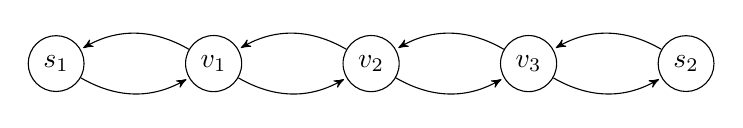
\begin{tikzpicture}
            [ auto
            , ->
            , >=stealth'
            , shorten >=1pt
            , node distance=2cm
            ]
            \node[mainNode] (1) {$s_1$};
            \node[mainNode] (2) [right of=1] {$v_1$};
            \node[mainNode] (3) [right of=2] {$v_2$};
            \node[mainNode] (4) [right of=3] {$v_3$};
            \node[mainNode] (5) [right of=4] {$s_2$};

            \path[every node/.style={font=\sffamily\small}]
            (1) edge [bend right] node {} (2)
            (2) edge [bend right] node {} (3)
            (3) edge [bend right] node {} (4)
            (4) edge [bend right] node {} (5)

            (5) edge [bend right] node {} (4)
            (4) edge [bend right] node {} (3)
            (3) edge [bend right] node {} (2)
            (2) edge [bend right] node {} (1)
            ;
        \end{tikzpicture}
\end{figure}

    \[
        P = 
        \bordermatrix{
           ~  & s_1 & v_1 & v_2 & v_3 &   s_2 \cr 
          s_1 &   0   & 1   & 0   & 0   & 0   \cr 
          v_1 &   0.5 & 0   & 0.5 & 0   & 0   \cr 
          v_2 &   0   & 0.5 & 0   & 0.5 & 0   \cr 
          v_3 &   0   & 0   & 0.5 & 0   & 0.5 \cr 
          s_2 &   0   & 0   & 0   & 1   & 0  
        }
    \] 
    \[
    \begin{split} 
        (0,0,1,0,0) P   & = (0,0.5,0,0.5,0) \\
        (0,0,1,0,0) P^2 & = (0.25,0,0.5,0,0.25) \\
        (0,0,1,0,0) P^3 & = (0,0.5,0,0.5,0)
    \end{split}
    \]
\end{frame}

\begin{frame}[t]
\frametitle{Absorbing Markov Chains}
Given a graph $G = (V, E)$: 
\begin{itemize}
	\item Remove edges between seed nodes.
	\item Replace edges by bi-directional arcs.
	\item For \highlight{seed nodes}: remove outgoing edges and 
		add a self-loop.
	\item For a non-seed node $u$, the probability associated with each 
		out-arc is $1/d(u)$.
\end{itemize}

    \begin{figure}
        \centering
        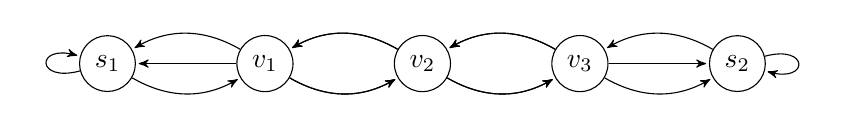
\begin{tikzpicture}
            [ auto
            , ->
            , >=stealth'
            , shorten >=1pt
            , node distance=2cm
            ]
            \node[mainNode] (1) {$s_1$};
            \node[mainNode] (2) [right of=1] {$v_1$};
            \node[mainNode] (3) [right of=2] {$v_2$};
            \node[mainNode] (4) [right of=3] {$v_3$};
            \node[mainNode] (5) [right of=4] {$s_2$};


            \uncover<1>{
            \path[every node/.style={font=\sffamily\small}]
            (1) edge [bend right] node {} (2)
            (2) edge [bend right] node {} (3)
            (3) edge [bend right] node {} (4)
            (4) edge [bend right] node {} (5)

            (5) edge [bend right] node {} (4)
            (4) edge [bend right] node {} (3)
            (3) edge [bend right] node {} (2)
            (2) edge [bend right] node {} (1)
            ;
            }
            \uncover<2->{
            \path[every node/.style={font=\sffamily\small}]
            %(1) edge [loop left]  node {} (1)
            %(5) edge [loop right] node {} (5)

            (2) edge [bend right] node {} (3)
            (3) edge [bend right] node {} (4)
            (4) edge node {} (5)

            (4) edge [bend right] node {} (3)
            (3) edge [bend right] node {} (2)
            (2) edge node {} (1)
            ;
            }

            \uncover<3->{
            \path[every node/.style={font=\sffamily\small}]
            (1) edge [loop left]  node {} (1)
            (5) edge [loop right] node {} (5)

            %(2) edge [bend right] node {} (3)
            %(3) edge [bend right] node {} (4)
            %(4) edge node {} (5)

            %(4) edge [bend right] node {} (3)
            %(3) edge [bend right] node {} (2)
            %(2) edge node {} (1)
            ;
            }
        \end{tikzpicture}
    \end{figure}

    \uncover<4->{
    This defines an \highlight{absorbing Markov chain}.
    \begin{itemize}
        \item \highlight{Absorbing States}: no outgoing probabilities.
        \item \highlight{Transient States}: finite path to at least one absorbing state.
    \end{itemize}

    \vsp

    Use infinite random walks in this graph.
    }
\end{frame}

\begin{frame}[t]
\frametitle{Absorbing Markov Chains}
\begin{figure}
        \centering
        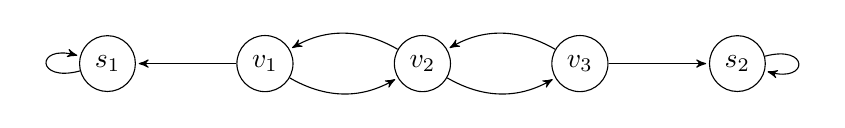
\begin{tikzpicture}
            [ auto
            , ->
            , >=stealth'
            , shorten >=1pt
            , node distance=2cm
            ]
            \node[mainNode] (1) {$s_1$};
            \node[mainNode] (2) [right of=1] {$v_1$};
            \node[mainNode] (3) [right of=2] {$v_2$};
            \node[mainNode] (4) [right of=3] {$v_3$};
            \node[mainNode] (5) [right of=4] {$s_2$};

            \path[every node/.style={font=\sffamily\small}]
            (1) edge [loop left]  node {} (1)
            (5) edge [loop right] node {} (5)

            (2) edge [bend right] node {} (3)
            (3) edge [bend right] node {} (4)
            (4) edge node {} (5)

            (4) edge [bend right] node {} (3)
            (3) edge [bend right] node {} (2)
            (2) edge node {} (1)
            ;
            ;
        \end{tikzpicture}
    \end{figure}

    \uncover<1->{
    \[
    P =
    \bordermatrix
        {
           ~  & v_1 & v_2 & v_3 & s_1 &   s_2 \cr 
          v_1 & 0   & 0.5 & 0   & 0.5 &   0   \cr
          v_2 & 0.5 & 0   & 0.5 & 0   &   0   \cr
          v_3 & 0   & 0.5 & 0   & 0   &   0.5 \cr 
          s_1 & 0   & 0   & 0   & 1   &   0   \cr
          s_2 & 0   & 0   & 0   & 0   &   1
        }
    =
    \begin{pmatrix}
	\begin{array}{c|c}
        Q & R \\ \hline 
        0 & I
	\end{array}
    \end{pmatrix}
    \] }
\end{frame}

\begin{frame}[t]
\frametitle{Constructing the Absorbing Markov Chain}
$$
	P =
      \begin{pmatrix}
	  \begin{array}{c|c}
        Q & R\\ \hline
        0 & I
	  \end{array}
      \end{pmatrix}
      ,\text{with}~
    P_{ij} =\begin{cases}
        \frac{1}{deg(v_i)}, & \text{if $(v_i,v_j) \in E$} \\
        0, & \text{otherwise}
        \end{cases}
    $$

    \vsp
    \vsp

    
    We can write $Q$ as 
    $$Q = D_1^{-1}A_1.$$

    where
    \begin{itemize}
        \item $A_1$ is adjacency matrix of graph induced by the non-seed nodes.
        \item $D_1$ is diagonal matrix with $D_{ii} = deg(v_i)$ for each non-seed node $v_i$.

    \end{itemize}
\end{frame}

\begin{frame}[t]
\frametitle{Absorbing Markov Chains~$\ldots$}
Powers of $P$:
    \[
    P =
    \begin{pmatrix}
	\begin{array}{c|c}
        Q & R \\ \hline
        0 & I
	\end{array}
    \end{pmatrix}
    ~~~
    P^k =
    \begin{pmatrix}
	\begin{array}{c|c}
        Q^k & \sum\limits_{i=0}^{k-1} Q^{i} R \\ \hline
        0   & I
	\end{array}
      \end{pmatrix}
    \]

    \uncover<2->
    {
    We define:
    $$P^\infty := \lim \limits_{k \rightarrow \infty}{P^k}$$
    }

    \uncover<3->
    {
    In absorbing Markov chains (without proof):
    $$
        P^\infty=
        \begin{pmatrix}
		\begin{array}{c|c}
            0 & (I-Q)^{-1}R \\ \hline
            0 & I
		\end{array}
          \end{pmatrix}
    $$
    }

    \uncover<4->
    {
    The probability that a non-seed vertex $v_i$ is 
	absorbed at a seed vertex $s_j$ equals the $ij$th entry 
	in $(I-Q)^{-1}R$.
    }
\end{frame}

\begin{frame}[t]
\frametitle{Estimating Affinity Vectors}
$E_{v \to s} := $ Event that infinite random walk (in modified graph) starting at $v$ gets trapped at $s$.

$$ (\alpha_1(v), \dots, \alpha_l(v)) := \sum_{s \in S} \Pr(E_{v \to s}) (\alpha_1(s), \dots, \alpha_l(s))$$

\medskip

$\Pr(E_{v \to s})$ corresponds to an entry in $P^\infty$.

\medskip

How do we calculate the entries of $P^\infty$ efficiently?
\end{frame}

\begin{frame}[t]
\frametitle{Symmetric Diagonally Dominant (SDD) Linear Systems}
We want to discover communities one by one. 
\begin{itemize}
	\item Fix a community $c$.
	\item Let $X := (I-Q)^{-1}R$. The affinities of non-seed nodes to 
	community $c$ is given by the column vector:
	\[
		Y_c = \sum_{s \in S} \alpha_c(s) \cdot X_{* s}
	\]
\end{itemize}

Write $Y_c$ as:
\begin{align*}
	Y_c & = \sum_{s \in S} \alpha_c(s) \cdot X_{* s} = \sum_{s \in S} \alpha_c(s) \cdot (I - Q)^{-1} R_{* j} \\
		& = (I - Q)^{-1} \sum_{s \in S} \alpha_c(s) \cdot R_{* j}. 
\end{align*}
\end{frame}

\begin{frame}[t]
\frametitle{SDD Systems}
\[
	(I - Q) Y_c = \sum_{s \in S} \alpha_c(s) \cdot R_{* j}.
\]

Since $Q = D_1^{-1} A_1$, 
\begin{itemize}
	\item $A_1$ is the adjacency matrix of the graph induced by non-seed nodes;
	\item $D_1(v, v) = d(v)$ for non-seed nodes $v$. 
\end{itemize}

We obtain the following SDD system:
\[
	(D_1 - A_1) Y_c = D_1 \sum_{s \in S} \alpha_c(s) \cdot R_{* j}.
\]
The rhs can be computed in $O(n)$ time since $R$ has only $O(n)$ non-zero entries. 

\medskip

\end{frame}

\begin{frame}[t]
\frametitle{Running Time}
SDD systems can be solved in nearly $O(m \log n)$ time (hides a factor of $(\log \log n)^2$). 
\begin{itemize}
	\item Spielman and Teng, \emph{Nearly linear-time algorithms for preconditioning
		and solving symmetric, diagonally dominant linear systems}, Preliminary version 
		in STOC 2004.
	
	\item Koutis, Miller and Peng, \emph{Approaching optimality for solving SDD systems}, 
		FOCS, 2010.

	\item Koutis, Miller and Peng, \emph{A nearly $O(m \log n)$-time solver for SDD systems}, 
		FOCS, 2011.
	
	\item Vishnoi, \emph{Laplacian Solvers and their Algorithmic Applications}, 2013.
\end{itemize}

Assuming $m = O(n)$, we take $O(n \log n)$ per community. The total time taken is
\[
	O(k \cdot n \log n),
\]
where $k$ is the number of communities.
\end{frame}

\end{document}
